\documentclass[a4paper,footsepline]{scrartcl}

\usepackage[utf8]{inputenc}
\usepackage[T1]{fontenc}
\usepackage{lmodern}

%##### English
\usepackage[english]{fancyref}
\usepackage[USenglish]{babel}

%#### Deutsch
%\usepackage[ngerman]{babel}
%\usepackage[german]{fancyref}

%#### Usepackage #####

\usepackage{uepage} 
\usepackage{amssymb}

\usepackage{courier}
\usepackage{hyperref}
\usepackage{listings}
\usepackage{color}
\usepackage{tikz}
\usepackage{wasysym}
\usepackage{framed}
\usetikzlibrary{arrows, automata}
\usepackage{ marvosym }


\newcommand{\vect}[1]{\begin{pmatrix} #1\end{pmatrix}}

\areaset{15cm}{26cm}

%#### Title page #####
\title{Cyber Physical Systems: Stochastic foundations UE}
\subject{Excercise 1}

\author{
	\authorname{Mathias Lechner and Benjamin Binder} \\
	\studentnumber{1225134, 1226121} \\
	\curriculum{066 938}\\
	\email{e1225134@student.tuwien.ac.at, e1226121@student.tuwien.ac.at}\\\\
}
\date{\today}


%### Start of Document
\begin{document}

\newcommand{\fcl}[1]{{\footnotesize#1\vspace{0.4cm}\\}}
\newcommand{\fclc}[2]{{\footnotesize#1\hspace{0.4cm}{\footnotesize #2}\vspace{0.4cm}}\\}
\newcommand{\mmatrix}[1]{\left [ \begin{matrix}#1\end{matrix} \right ]}
\newcommand{\SpaceEx}[0]{\textsc{SpaceEx} }

%% vector
\newcommand{\vc}[1]{\ensuremath{\boldsymbol{\lowercase{#1}}}}

%% matrix
\newcommand{\mt}[1]{\ensuremath{\boldsymbol{\uppercase{#1}}}}

%% random vector
\newcommand{\rvc}[1]{\ensuremath{\text{\sffamily\bfseries\lowercase{#1}}}}

%% random matrix
\newcommand{\rmt}[1]{\ensuremath{\text{\sffamily\bfseries\uppercase{#1}}}}

%% random variable
\newcommand{\rv}[1]{\ensuremath{\text{\sffamily\lowercase{#1}}}}

%\newcommand{\rv}[1]{\mathrm{#1}}
%\newcommand{\rvv}[1]{\bm{\mathrm{#1}}}
\newcommand{\dv}[1]{\mathit{#1}}
\newcommand{\dvv}[1]{\bm{\mathit{#1}}}
\newcommand{\pdf}[1]{f_\rv{#1}(\dv{#1})}
\newcommand{\pdfa}[2]{f_\rv{#1}(\dv{#2})}
%\newcommand{\cdf}[1]{F_\rv{#1}(\dv{#1})}
\newcommand{\cdf}[2]{F_\rv{#1}(\dv{#2})}
\newcommand{\prob}[1]{\mathrm{P}\{#1\}}
\newcommand{\pmf}[1]{p_\rv{#1}(\dv{#1})}
	
	\maketitle
	\section*{Task 1.1: Intelligent Agents}
	A robot, equipped with several sensors, should autonomously navigate through a world. A
	start and goal position will be given. The world only contains static objects, i.e., the only
	moving object is the robot.\\
	A mars rover should transport goods between two base stations. The rover is the only one of its kind on mars, i.e. no other movable object is assumed to be encountered on its mission.  The rover has four wheels, each equipped with a electrical motor and a brake.
	The front-axie is used for steering and the steering is controlled by a motor. The world consists of sandy  terrain and craters, the robot should not drive into a crater. Close to the two base stations, space ships and other static objects are placed and should avoided. The robot is equipped with state of the art sensors for autonomous driving. The robot is connected to a satellite which monitors the trip of the rover and may send correction data of the position of the rover.
	\begin{description}
		\item[Performance measure]
		Reach goal position
		\item[Environment]
		Sandy terrain, craters, Static objects
		\item[Actuators]
		Motors for acceleration and steering angle, brake
		\item[Sensors]
		INS, position from satellite, Lidar, Camera, Wheel rotation, Steering angle
	\end{description}
	\vspace{0.3cm}
	\begin{tabular}{|lr|lr|}\hline
		fully observable & \Square & partially observable & \CheckedBox \\\hline
		single agent & \CheckedBox & multiple agent & \Square \\\hline
		deterministic & \Square & stochastic & \CheckedBox \\\hline
		static  & \CheckedBox & dynamic & \Square \\\hline
		discrete & \Square & continuous & \CheckedBox \\\hline
	\end{tabular}
	\section*{Task 1.2: Stochastic Basics - Discrete Random Variables}
	a) Show that $P(a | b \land a) = 1$
	\begin{align*}
	P(a | b \land a) & = \frac{P(\{b \land a\} \cap a)}{P(b \land a)}\\
	& = \frac{P(b \land a)}{P(b \land a)}\\
	& = 1
	\end{align*}
	\vspace{0.4cm}\\
	b) Prove that if two random variables x and y are independent (denoted by x $\bot$ y), they are
	also uncorrelated.
	\vspace{0.1cm}\\
	First we will compute the correlation $R_{x,y}$ of $x$ and $y$:
	\begin{align*}
		R_{x,y} &= \int_{-\infty}^{\infty} \int_{-\infty}^{\infty}  x y f_{x,y}(x,y)\ \text{d} x\ \text{d} y\\
		&= \int_{-\infty}^{\infty} \int_{-\infty}^{\infty}  x y f_x(x) f_y(y)\ \text{d} x\ \text{d} y\\
		&= \int_{-\infty}^{\infty} y f_y(y) \underbrace{ \int_{-\infty}^{\infty}  x f_x(x) \ \text{d} x}_{= \mu_x} \ \text{d} y\\
		&= \int_{-\infty}^{\infty} y f_y(y)\mu_x\ \text{d} y\\
		&= \mu_x \underbrace{\int_{-\infty}^{\infty} y f_y(y)\ \text{d} y}_{= \mu_y}\\
		&= \mu_x \mu_y
	\end{align*}
	So we get the covariance: $C_{x,y} = R_{x,y} - \mu_x \mu_y =0$, \\
	 thus  $x$ and $y$ are uncorrelated.
	 \vspace{0.4cm}\\
	c) Give an example where two random variables x and y are uncorrelated but not independent.
	\vspace{0.1cm}\\
	Let $x,y$ be two discrete random variables with probability: 
	\begin{align*}
		P(0,1) &= \frac{1}{2}\\
		P(1,-1) &= \frac{1}{4}\\
		P(-1,-1) &= \frac{1}{4}
	\end{align*}
	Obviously $\mu_x = \mu_y = 0$.
	With correlation:
	\begin{align*}
	R_{x,y} &= \int_{-\infty}^{\infty} \int_{-\infty}^{\infty}  x y f_{x,y}(x,y)\ \text{d} x\ \text{d} y\\
	&= 0 \cdot 1 \cdot \frac{1}{2} + 1 \cdot (-1) \cdot \frac{1}{4} + (-1) \cdot (-1) \cdot \frac{1}{4}\\
	&= - \frac{1}{4} +  \frac{1}{4}\\
	&= 0
	\end{align*}
	which equals $\mu_x \cdot \mu_y$, i.e. $x$ and $y$ are uncorrelated.\\
	But $x$ and $y$ are not independent, shown by the counterexample:
	\[ f_{x,y}(0,1) = \frac{1}{2} \]
	\[ f_x(0) \cdot f_y(1) = \frac{1}{2} \cdot \frac{1}{2} =\frac{1}{4}  \]
	\vspace{0.4cm}\\
	d) If $x$ and $y$ are normally distributed and independent with the same variance ($x \sim  \mathcal{N}(\mu_x, \sigma)$ and $y \sim  \mathcal{N}(\mu_x, \sigma)$ and $x \bot y$), prove that $x-y$ and $x+y$ are independent.
	\vspace{0.2cm}\\
	We have the covariance matrix of $x$ and $y$ of:
	\begin{align*}
		C_{x,y} &= \vect{\sigma_x^2 & C_{x,y}\\C_{y,x} & \sigma_y^2}\\
		&=\vect{\sigma^2 & 0 \\0 & \sigma^2}
	\end{align*}
	Note: $C_{x,y} = C_{y,x} = 0$ because $x$ and $y$ are independent.\vspace{0.2cm}\\
	Let $v = x + y$ and $w=x-y$, i.e. we get the linear transformation matrix $A$:
	\[ \vect{v\\w} = \vect{ 1 & 1 \\ 1 & -1} \cdot \vect{x\\y} \] 
	Thus giving us the transformed covariance matrix:
	\begin{align*}
		C_{v,w} &= A\ C_{x,y}\ A^T\\
		&= \vect{ 1 & 1 \\ 1 & -1}\ \vect{\sigma^2 & 0 \\0 & \sigma^2}\ \vect{1 & 1\\1 & -1}\\
		&= \vect{\sigma^2 & \sigma^2\\\sigma^2 & -\sigma^2} \ \vect{1 & 1\\1 & -1}\\
		&= \vect{2 \sigma^2 & 0\\0 & 2 \sigma^2}
	\end{align*}
	Thus, $v$ and $w$ are uncorrelated.\\
	Next we will use the two theorems two show independence:\\
	\begin{framed}
		1) A linear transformed normal distributed and independent vector is also normally distributed (but not necessarily independent).
	\end{framed}
	\begin{framed}
		2) For two jointly normal distributed variables it hold that: Independent = Uncorrelated
	\end{framed}
	Thus $\vect{v\\w}$ is a uncorrelated normal distributed vector, therefore $v$ and $w$ are independent.
	\section*{Task 1.3: Stochastic Basics - Continuous Random Variables}
	The random variable $t$ represents the duration until system $S$ fails. The probability density
	function (pdf) $f_t(t)$ is:
	\[f_t(t) = \begin{cases} 
	\lambda e^{-\alpha t} & t \geq 0\\
	0 & t < 0
	\end{cases} \qquad \text{where } \alpha=\frac{1}{5 \text{ years}} \]
	a) Calculate $\lambda$, sketch the pdf $f_t(t)$ and give the cdf.
	\begin{align*}
		\int_{-\infty}^{\infty} f_t(t) &= 1\\
		\int_{0}^{\infty} \lambda e^{-\alpha t} &= 1\\
		\Big[ \lambda \frac{e^{-\alpha t}}{- \alpha}\Big]_0^\infty &= 1 \\
		\lambda \frac{e^{-\alpha \infty}}{- \alpha} - 	\lambda \frac{e^{-\alpha 0}}{- \alpha} &= 1 \\
		\lambda \frac{1}{\alpha} &= 1 \\
		\lambda &= \alpha
	\end{align*}
	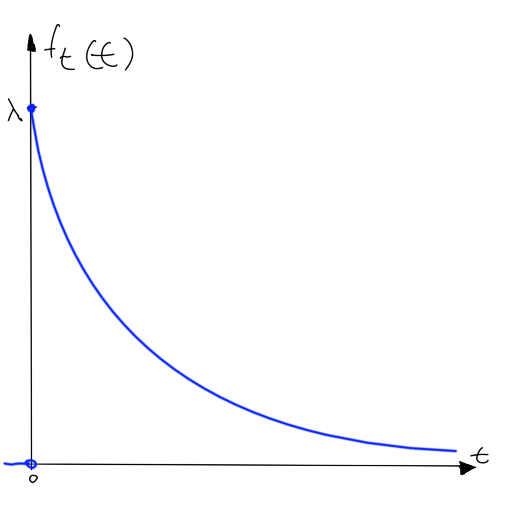
\includegraphics[width=\textwidth]{sketch.png}
	\begin{align*}
	F_{t \geq 0}(t) &= \int_{0}^{t} f_t(\tau)\ \text{d} \tau \\
	&= \int_{0}^{t} \alpha e^{-\alpha \tau}\ \text{d} \tau\\
	&= 	\Big[ \alpha \frac{e^{-\alpha \tau}}{- \alpha}\Big]_0^t\\
	&= - e^{-\alpha t} + e^{-\alpha 0}\\
	&= 1-e^{-\alpha t}
	\end{align*}
	Altogether:
	\[ F_t(t) = \begin{cases} 1-e^{-\alpha t} & t \geq 0\\
	0 & t < 0
	\end{cases} \]
	\vspace{0.4cm}\\
	b) Calculate the Mean Time To Failure (MTTF) of system S.\\
	\begin{align*}
		\mu_t &= \int_{-\infty}^{\infty} t\ f_t(t)\ \text{d} t\\
		&= \int_{0}^{\infty} t\ \alpha\ e^{-\alpha t}\ \text{d} t\\
		&= \Big[ t\ \alpha\  \frac{e^{-\alpha t}}{- \alpha}  \Big]_0^\infty - \int_{0}^{\infty} \alpha\ \frac{e^{-\alpha t}}{- \alpha}\ \text{d} t\\
		&=  \lim\limits_{t \rightarrow \infty} - t\  e^{-\alpha t} + 0\ e^{- \alpha\ 0} - \big[ \frac{e^{-\alpha t}}{\alpha}\ \Big]_0^\infty \\
		&= - \lim\limits_{t \rightarrow \infty} \frac{e^{-\alpha t}}{\alpha}  + \frac{e^{-\alpha 0}}{\alpha}\\
		&= \frac{1}{\alpha}\\
		&= 5 \text{ years}
	\end{align*}
	c) Calculate the probability that system $S$ does not fail in the first 3 years.\\
	\begin{align*}
	 P(t \geq 3) & = 1 - P(t < 3) = 1 - F_t(3) \\
	 &= 1 - 1  + e^{-\alpha 3}\\
	 &= e^{-\frac{3}{5}} \\
	 & \approx 55\%
	\end{align*}
	d) What is the probability that system $S$ didn’t fail within the first 3 years, but does so
	between 5 and 7 years?
	\begin{align*}
		P(5 \leq t \leq 7 | t \geq 3) &= \frac{P(\{5 \leq t \leq 7\} \cap \{t \geq 3\} ) }{P(t \geq 3)}\\
		&= \frac{P(5 \leq t \leq 7)}{P(t \geq 3)}\\
		&= \frac{F_t(7) - F_t(5)}{1-F_t(3)}\\
		&= \frac{\big(1-e^{-\frac{7}{5}}\big) - \big(1-e^{-\frac{5}{5}}\big)}{1-\big(1-e^{-\frac{3}{5}}\big)}\\
		&= \frac{e^{-\frac{5}{5}}-e^{-\frac{7}{5}}}{e^{-\frac{3}{5}}}\\
		&\approx 22\%
	\end{align*}
	e) System S has been upgraded. The new system $S$ cannot fail in the first 3 years anymore,
	but it might fail exactly after 3 years with the probability p. After this point the time
	to failure behaves as before.\\
	i) What is the probability $p$?\\
	\[ p = 1 - P(t > 3) = P(t \leq 3) = F_t(3) = 1 - e^{-\frac{3}{5}} \approx 0.45119 \dots \]
	ii) Give a pdf $f_ x(x)$ that models failure over time of the upgraded system. Also sketch
	the pdf of $x$.\\
	\[f_t(t) = \begin{cases} 
	p\ \delta(t-3) + \lambda e^{-\alpha t} & t \geq 3\\
	0 & t < 3
	\end{cases} \qquad \text{where } \delta(t) \text{ is the dirac distribution} \]
	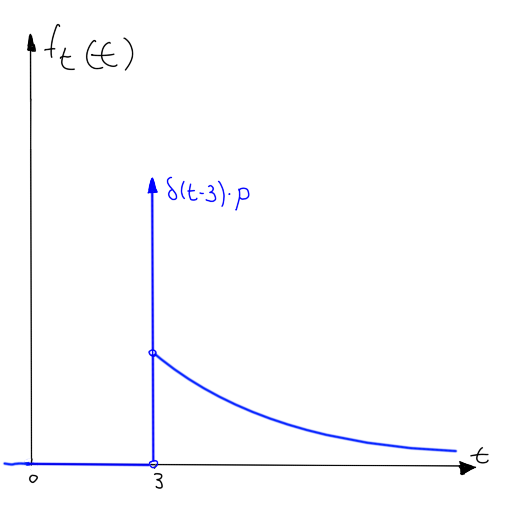
\includegraphics[width=\textwidth]{sketch2.png}
	iii) Repeat subtask d) for the upgraded system.\vspace{0.2cm}\\
	What has changed is that $P(t < 3)=0$ which implies that:\\ 
	\[P(t \geq 3) = 1-P(t < 3) = 1-0 =1\]
	For the conditional probability that gives us:
	\begin{align*}
	P(5 \leq t \leq 7 | t \geq 3) &= \frac{P(\{5 \leq t \leq 7\} \cap \{t \geq 3\} ) }{P(t \geq 3)}\\
	&= \frac{P(5 \leq t \leq 7)}{1}\\
	&= P(5 \leq t \leq 7)\\
	&= F_t(7) - F_t(5)\\
	&=\big(1-e^{-\frac{7}{5}}\big) - \big(1-e^{-\frac{5}{5}}\big)\\
	&= e^{-\frac{5}{5}}-e^{-\frac{7}{5}}\\
	&\approx 12\%
	\end{align*}
	\section*{Task 1.4: Bayes Nets - Conditional Probabilities}
	In your local nuclear power station, there is an alarm that senses when a
temperature gauge exceeds a given threshold. The gauge measures the temperature
of the core. Consider the Boolean variables $\rv{a}$ (alarm sounds), $\rv{f}_a$
(alarm is faulty), and $\rv{f}_g$ (gauge is faulty) and the continuous
variables $\rv{g}$ (gauge reading) and $\rv{t}$ (actual core temperature).

a) Draw a Bayesian network for this domain, given that the gauge is more
  likely to fail when the core temperature gets too high.
	\begin{figure}[h]
	 \centerline{
		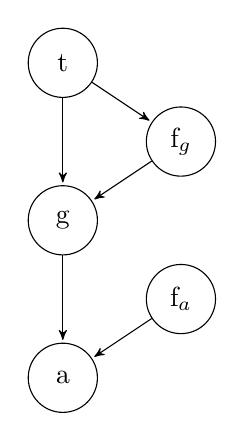
\begin{tikzpicture}[>=stealth',shorten >=1pt,auto,node distance=4cm]
		  \node[state] (t)    at (3,0)       {t};
		  \node[state] (f_g)   at (4.5,-1)      {f$_g$};
		  \node[state] (g)   at (3,-2)       {g}; %node at (4,0.9) {$p_0 \in CS$};
		  \node[state] (f_a) at (4.5,-3) {f$_a$};
		  \node[state] (a) at (3,-4) {a};
		  \path[->]  (t)  edge (g);
		  \path[->]  (t)  edge (f_g);
		  \path[->]  (f_g)  edge (g);
		  \path[->]  (g)  edge (a);
		  \path[->]  (f_a)  edge (a);
		\end{tikzpicture}
	  }
	  \caption{Bayesian network for the given domain}
	  \label{fig:bayes}
	\end{figure}

b) Suppose there are just two possible actual and measured temperatures,
  $normal$ and $high$; the probability that the gauge gives the correct
  temperature is $x$ when it is working, but $y$ when it is faulty. Give the
  conditional probability table associated with $\rv{g}$.

	\vspace{0.5cm}
	\begin{tabular}{|c|c|c|c|}\hline
		$\rv{f}_g$ & $\rv{t}$ &  $\rv{g}$  & $P(\rv{g}|\rv{f}_g,\rv{t})$ \\\hline
		false      & $normal$ &  $normal$  & x \\\hline
		false      & $high$   &  $high$    & x \\\hline
		true       & $normal$ &  $normal$  & y \\\hline
		true       & $high$   &  $high$    & y \\\hline
	\end{tabular}
	\vspace{0.5cm}

c) Suppose the alarm works correctly unless it is faulty, in which case it
  never sounds. Give the conditional probability table associated with
  $\rv{a}$.
  
  	\vspace{0.5cm}
  	\begin{tabular}{|c|c|c|c|}\hline
		$\rv{f}_a$ & $\rv{g}$   &  $\rv{a}$ & $P(\rv{a}|\rv{f}_a,\rv{g})$ \\\hline
		false      & $normal$   &  false    & x \\\hline
		false      & $high$     &  true     & x \\\hline
		true       & $normal$   &  false    & y \\\hline
		true       & $high$     &  false    & y \\\hline
	\end{tabular}
	\vspace{0.5cm}

d) Suppose the alarm and gauge are working and the alarm sounds. Calculate
  an expression for the probability that the temperature of the core is too
  high, in terms of the various conditional probabilities in the network.


	
\end{document}